\chapter{设计与实现 }
\label{ch3}

\section{系统功能介绍}
本文以帮助研究人员和开发人员了解Android应用程序的执行过程作为基本出发点,通过设计与实现Android动态函数调用图构建系统RunDroid,生成Android应用程序运行时对应的动态函数调用图,从方法调用关系、方法间的触发关系以及方法执行的相关对象信息等多个方面较为全面地展现Android应用的执行过程,为应用程序分析提供更为多样、准确的信息。另外,系统具备一定的可拓展性,可以方便相关人员根据自身的业务需求对系统进行扩展,完成相应的需求。

\section{基本思想}



\begin{figure*}[ht]
	\centering
	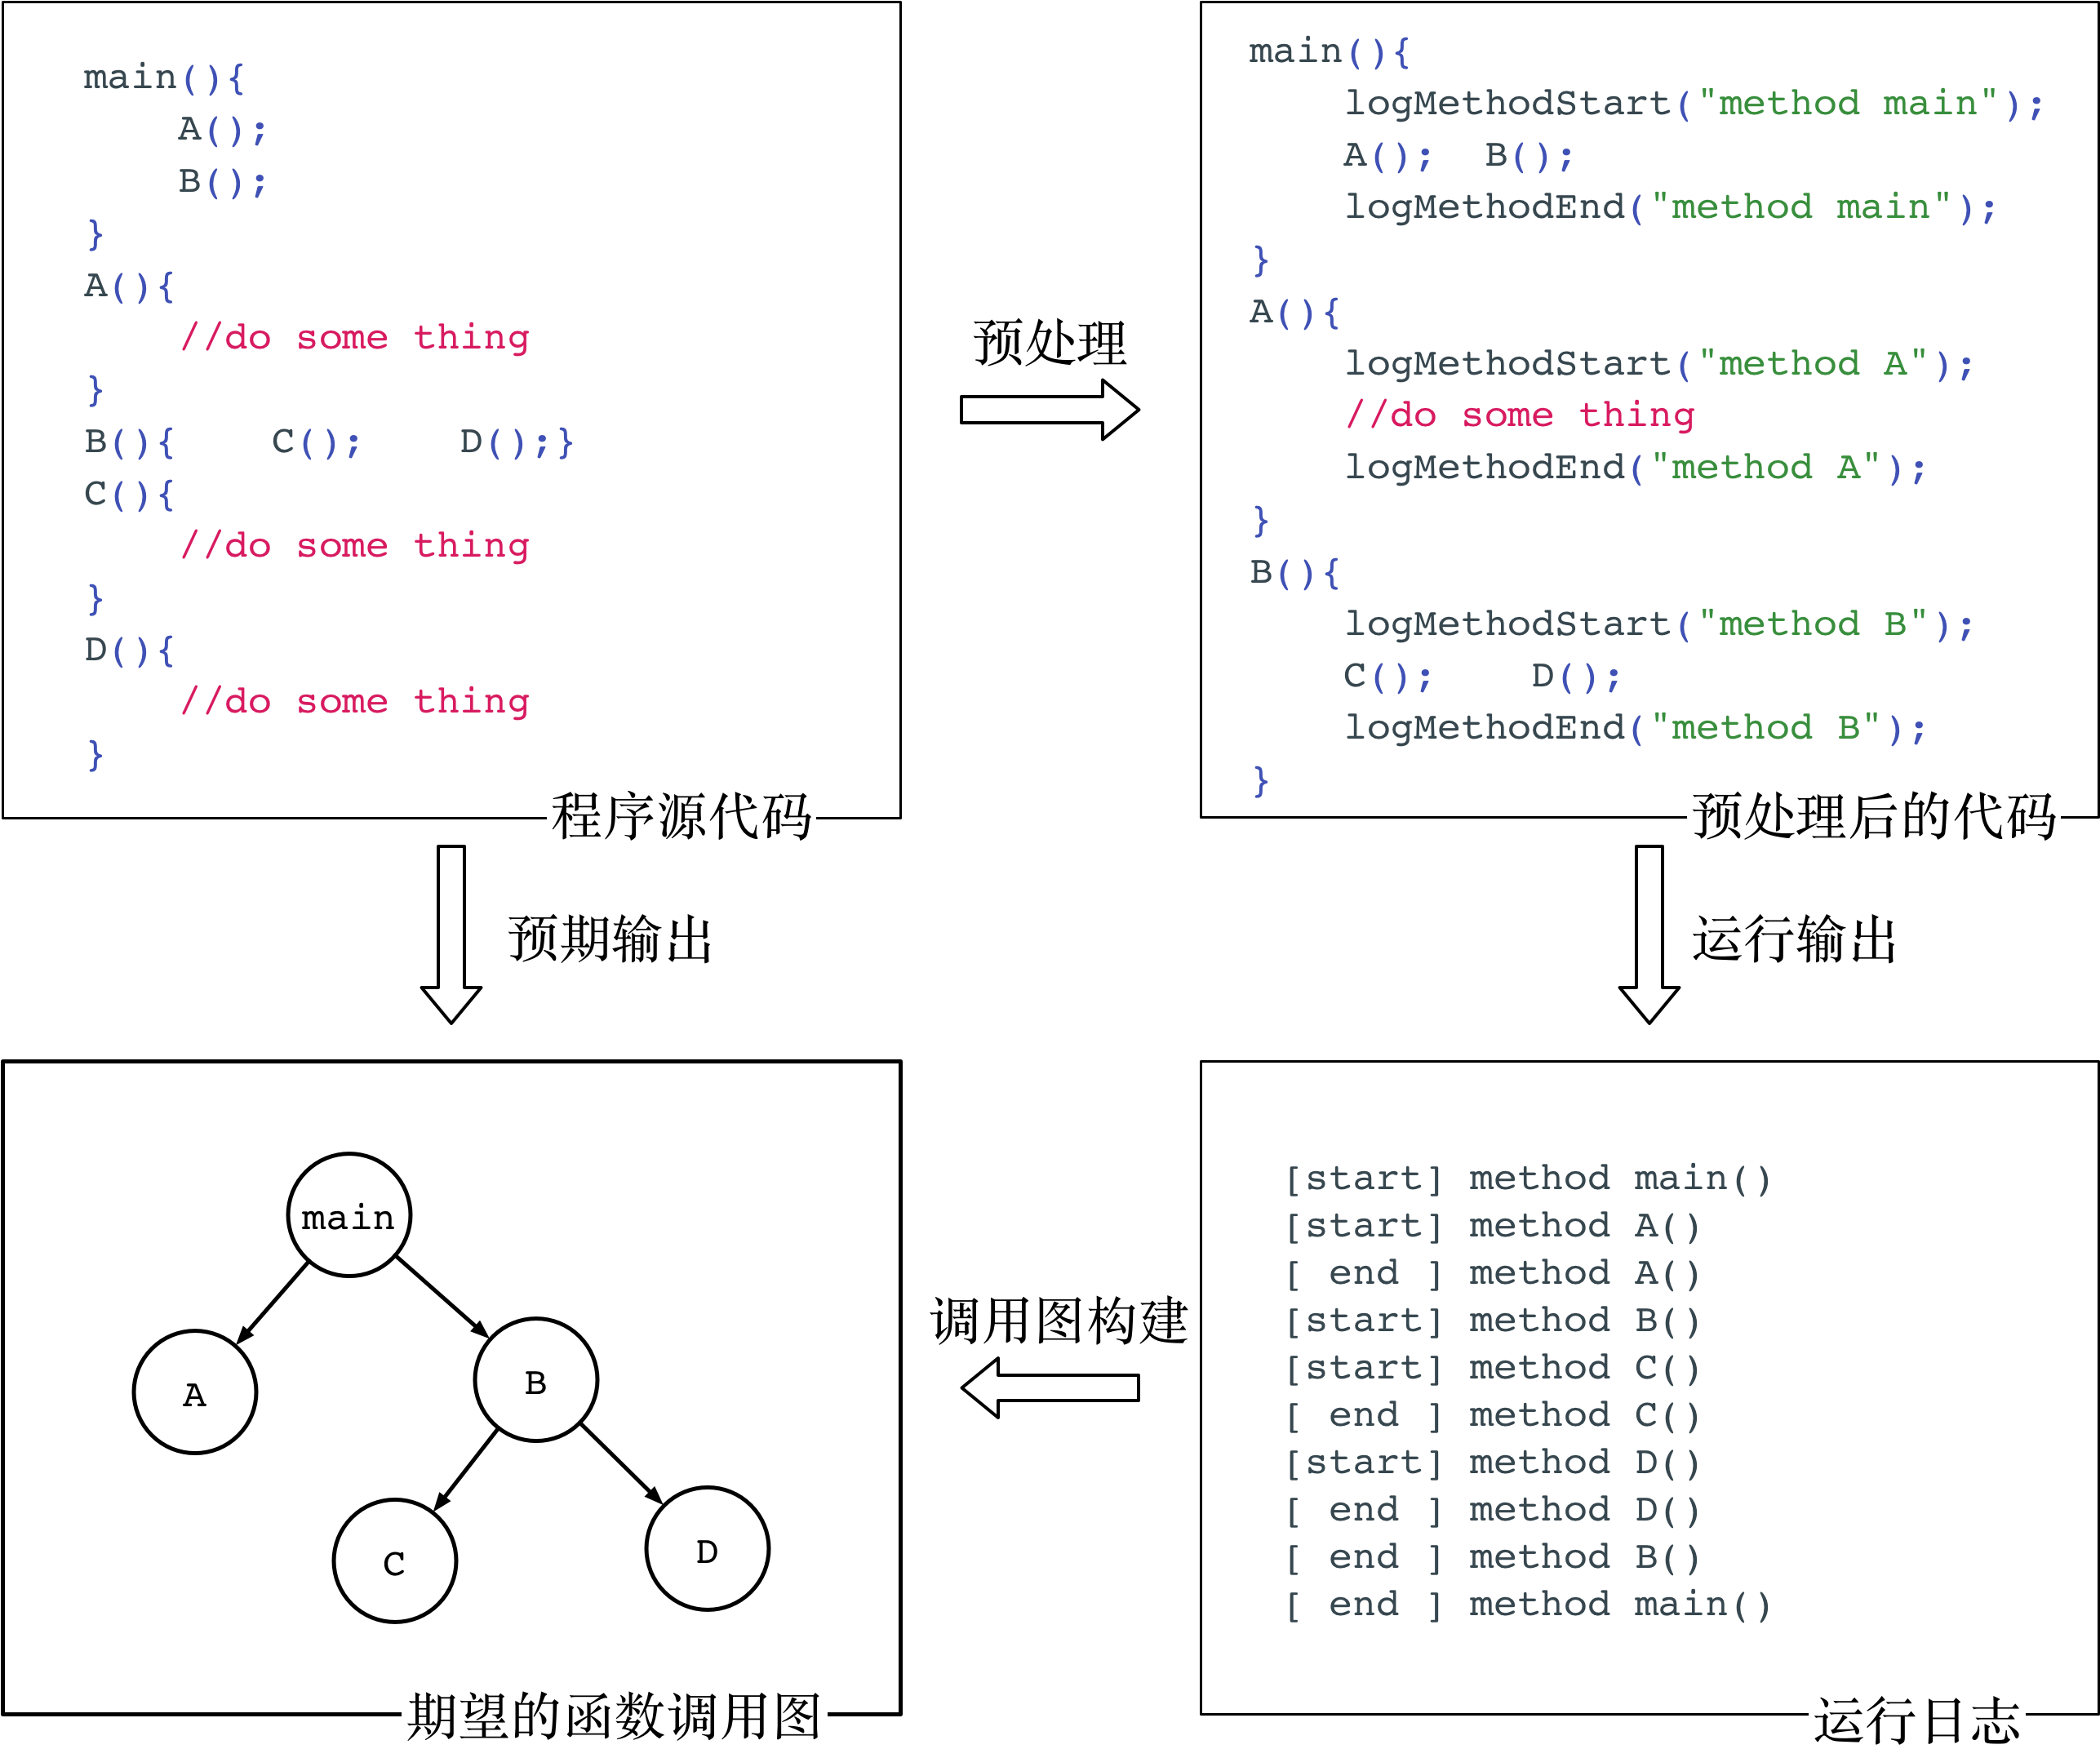
\includegraphics[width=\textwidth]{./Figures/code-sample.png}
	\caption{RunDroid的基本思路}
	\label{fig:code_sample}
\end{figure*}


%在本节,
以~\autoref{fig:code_sample}为例,%简要介绍一下RunDroid还原Android应用程序的函数调用图的基本思路:
~\autoref{fig:code_sample}-左上为一段示例代码:在main函数执行时,程序会依次调用A、B两个函数,而B函数则会调用了C、D两个函数。
~\autoref{fig:code_sample}-左下则是期望输出——函数调用图。
在本质上,函数调用图属于树。程序执行过程可以看做树的深度优先遍历过程。
函数调用图还原的关键点,在于如何在程序执行过程中输出树的遍历序列,并根据遍历序列进行还原。
通常的,树的遍历分为中序遍历、前序遍历以及后序遍历三种。
不幸的,两颗结构完全不同的树对应的遍历序列可能是一样的,
这也就意味着上述三种遍历方法均不能直接还原出函数调用图。

若在程序执行前后均记录日志(即一个方法的执行会输出两条日志:方法开始日志、方法结束日志)时,
我们得到的遍历序列是唯一的,可以直接用于函数调用图的还原。
% 而且,函数执行过程中出现的错误异常可能使得序列输出中断,阻碍调用图的构建。

为此,我们采用的基本思路如下:
通过对源程序(~\autoref{fig:code_sample}-左上)进行预处理,得到包含日志记录功能的运行代码(~\autoref{fig:code_sample}-右上);
程序在函数执行前后可以输出和方法执行相关的日志信息,(~\autoref{fig:code_sample}-右下);
最后,我们根据这些日志信息构建出函数调用图(~\autoref{fig:code_sample}-左下)。
在函数调用图的基础上,RunDroid利用日志中包括的方法对象信息,挖掘和方法对象相关联的方法,结合具体触发规则,进而建立方法触发关系。

% 从函数调用图的构建过程可以看出,程序的执行过程就是对函数调用图自上而下的深度优先遍历过程。由此可见,若要还原出图 6-右中的函数调用图,本文采用的基本思路是以日志方式输出对右图中的函数调用图的深度优先遍历序列,并基于得到的遍历序列还原出函数调用图。
% 由于Android是由面向对象编程语言Java开发的系统,系统还需要考虑面向对象编程的特性——多态性(即同一个行为在不同的对象下的表现可以不同)。为此,RunDroid还会在函数调用图将函数执行和对应的对象进行关联,更好地体现面向对象编程的函数调用关系。基于上述的函数调用关系的信息,RunDroid根据函数调用之间的关系进一步挖掘,进一步挖掘Android系统中的特性(例如组件Activity的生命周期、多线程的交互方式)。

\section{技术路线}

在技术实现上,RunDroid主要分为预处理器、运行时拦截器、日志记录器、调用图构建器等4个部分。
对应技术路线如下:
预处理器通过源代码插桩技术实现用户方法层面的信息记录,而运行时拦截器则负责拦截系统方法的执行。
在应用运行时,日志记录器会记录用户方法和系统方法对应的执行信息,以日志的形式记录下来。
最后,调用图构建器会根据应用程序运行时输出的日志,构建拓展函数调用图。
对应的工作流程如~\autoref{fig:rundroid_overview}所示。


% 本技术路线拟利用语法分析工具,对Android应用程序进行了应用源代码层面的执行日志插桩工作,利用非侵入式系统行为修改插件获取系统层面的函数执行信息。
% 结合以上日志信息,方案对日志进行初步处理,在图数据库上构建原始的Android应用程序的动态函数调用图。
% 通过阅读分析Android系统中多线程相关的源代码,制定具体的多线程分析插件,进而在函数调用图中标识出多线程相关的方法间触发关系,
%全面地展现Android应用的执行过程。


\begin{figure*}[ht]
	\centering
	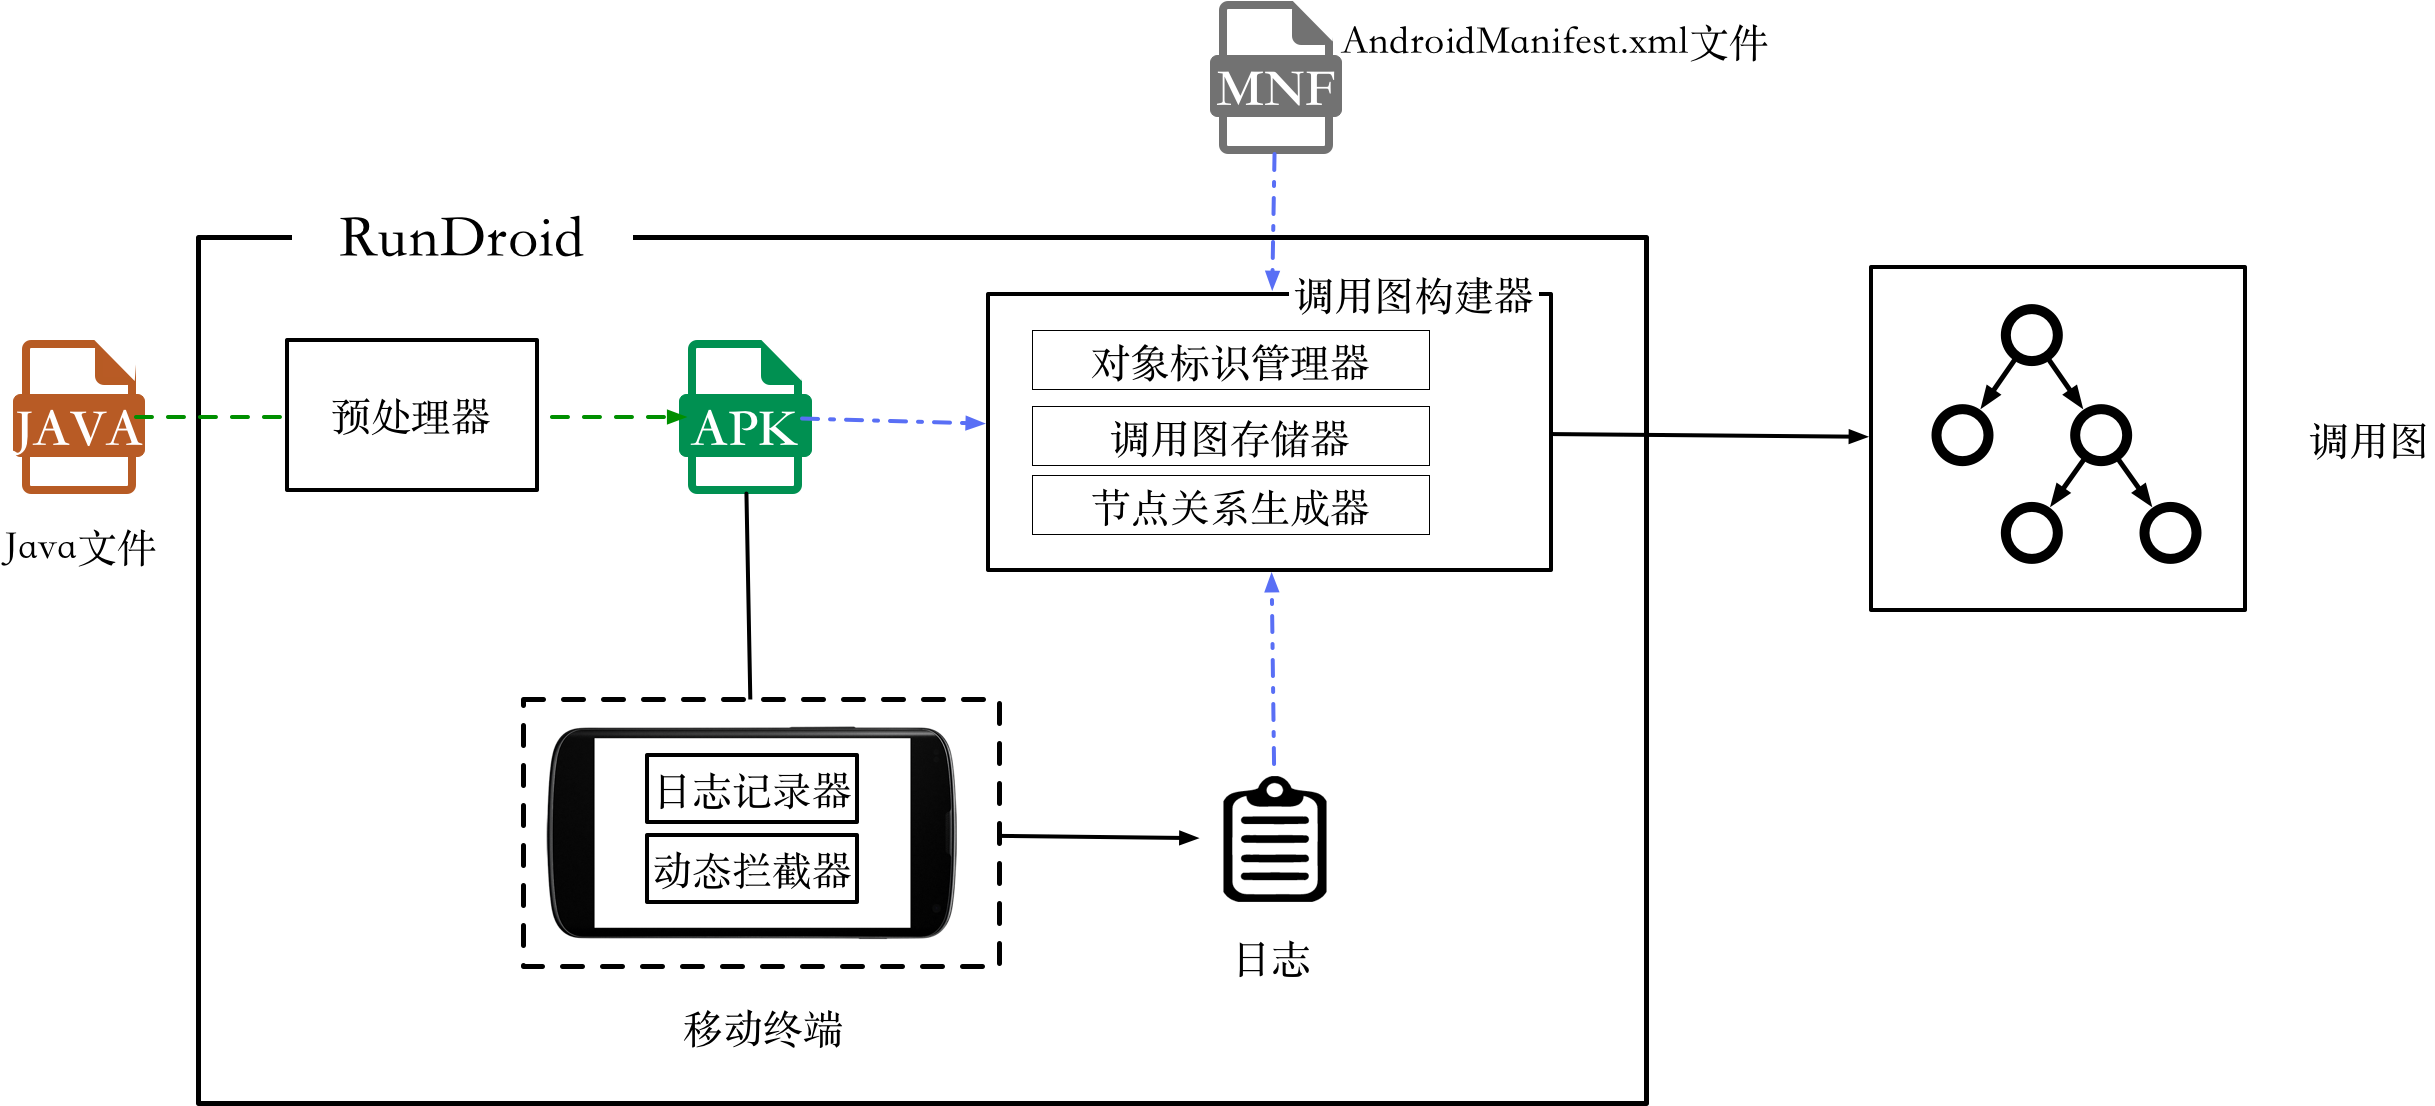
\includegraphics[height=0.5\textheight]{./Figures/rundroid-overview.png}
	\caption{ RunDroid的工作流程}
	\label{fig:rundroid_overview}
\end{figure*}


\section{相关技术介绍}


\subsection{srcML}
srcML~\cite{collard2013srcml}是轻量级源代码分析工具,它可以将程序的抽象语法树以XML的形式展现给用户,支持C、C++、C\#以及Java等多个语言的语法解析。
srcML的语法解析器采用的是基于LL(*)算法实现的语法解析器 ANTLR 2.7.7,解析得到的XML内容保留了源代码中完整的语法树信息。
同时,srcML还提供了一个强大工具集,支持对生成内容的查询、分析以及修改,可以用于架构设计、语言研究、软件重构等场景,应用于软件工程、编程语言、并行和分布式处理等多个领域。
在RunDroid,srcML承担的主要职责为源代码的语法解析,辅助完成用户方法层面的日志代码的编织(weaving)。



\subsection{Xposed框架}
Xposed~\cite{Xposed}是由rovo89主导开发的第三方框架。
基于Xposed开发的第三方插件,可以在不修改系统和应用程序源代码的情况下,改变他们的运行行为。
Xposed框架可以运行在不同版本的Android系统上,开发过程十分便利,而且易于撤销。
Xposed的实现原理具体如下:由于Android系统的所有的应用程序进程都是由Zygote进程孵化而来,Xposed通过替换程序\textit{/system/bin/app\_process},使得系统在启动过程中加载Xposed的相关文件,将所有的目标方法指向Native方法xposedCallHandler,维护目标方法和对应的钩子方法(Hook Function)的映射关系,从而实现对Zygote进程及Dalvik虚拟机的劫持;
当程序执行到目标方法时,xposedCallHandler会完成目标方法的原有代码和对应钩子方法的调度,达到对目标方法劫持的目的。
在RunDroid中,Xposed可以帮助我们实现类似面向切面编程(Aspect-Oriented Programming, AOP)的功能,辅助完成系统方法的执行情况的日志记录。
\subsection{Neo4j}
Neo4j~\cite{Neo4jthe19}是基于Java语言开发的图数据库。
与传统的基于关系模型的存储结构不同,Neo4j的存储模型是基于图论开发的,遵循属性图数据模型。
Neo4j的数据主要分为节点(Node)和关系(Relationship)两大类,分别对应图论中的点与边。
另外,Neo4j还可以在关系和节点上添加key-value形式的属性,为节点指定一个或者多个标签,为关系指定类型等等。
Neo4j以Lucence作为索引支撑,支持完整的 ACID(原子性,一致性,隔离性和持久性)事务规则,提供了基于Cypher脚本、Native Java API和REST Http API等多种方式帮助开发人员进行数据开发工作。
同时,Neo4j还提供了友好的浏览器界面,具有十分友好的交互体验。
由于基于属性图数据模型,Neo4j通常适用于和图关系有着密切关系的应用场景:例如社交网络分析,公共交通网络研究以及地图网络拓扑等场景。
在RunDroid,Neo4j主要承担着拓展函数调用图的数据存储和查询的主要职责。

\section{模块实现}


\subsection{预处理器}

为了捕获用户方法的运行时执行信息,RunDroid的预处理器组件会对应用程序进行插桩工作。
为了避免传统字节码插桩技术在生成过多的方法数而导致的方法数65K限制问题,预处理器采用的方案是源代码层面的插桩方案。
该方案通过源程序修改,将日志记录代码直接作用在方法体内部,最大限度地减少了APK构建过程中方法数的增加,避免了方法数65K限制问题。
日志记录代码在方法执行前后会调用日志记录器输出方法执行日志。


预处理器以Android项目源代码作为输入,输出预处理后的APK文件。
预处理器会遍历项目源代码中的每一个Java文件,利用srcML转化成对应的抽象语法树。
%  利用获取的语法结构,预处理器会提取出所有的方法体,
对于抽象语法树中的每一个方法,预处理器会计算出编译后所处的类的全限类名及对应的完整的方法签名,并将这些信息以日志记录代码的形式写回到方法体中。
另外,日志记录代码记录了和方法相关的方法对象信息:和方法有参数或者实例关系的对象会在方法执行时输出到日志,方法的返回值对象则是在方法结束以后输出到日志中。
%全限类名和方法签名的组合<全限类名,方法签名>和抽象语法树中的方法体一一对应,因此我们根据这些日志信息,定位到具体对应的方法体,还原出函数调用关系,构建出函数调用图。
另外,预处理器还对每个方法体进行了异常捕获处理,防止方法体内部的异常导日志记录过程的中断,影响函数调用图的构建。
最后,预处理器会将插桩后的源代码构建成APK文件。


% 为了捕获应用层中的方法调用,我们使用程序测试来记录运行时执行跟踪。在Java程序的源代码或字节码上有许多自动化的仪器工具(1)。
% 由于使用RunDood的上下文是在调试阶段,所以在源级对程序进行测试是很自然的。
% 此外,我们观察到字节码检测技术,如一个艾玛(3)使用,遭受64K参考限制[2 ]。
% 因此,预处理器组件建立在SRCML(9)上,它将Java源代码转换成XML格式,以便在执行过程中监视这些方法。


 \subsection{运行时拦截器}
 运行时拦截器的主要职责是对Android系统定义的方法执行进行拦截,将相关信息传递给日志记录器,弥补预处理器无法捕获系统方法执行信息的缺陷。
 运行时拦截器可以帮助提供系统方法的执行信息,填补调用图缺失的系统方法执行,进而可以还原出应用层和系统层之间以及系统内部的方法调用,进而帮助我们还原出方法间的触发关系。

在实现上,运行时拦截器是基于Xposed的插件,它维护的列表包括了所有需要拦截的系统方法,具体如~\autoref{tbl:hookMethodList} 所示。

\begin{table}
\caption{运行时拦截器拦截的系统方法列表}

\label{tbl:hookMethodList}

\begin{tabular}{|l|c|}
	\hline
	方法签名&说明\\
	\hline
	android.app.Activity onCreate android.os.Bundle   &\multicolumn{1}{c}{和Android Activity生命周期相关的方法}\\
%	\cline{1-1}
	android.app.Activity onStart    &\\
	android.app.Activity onResume    &\\
	android.app.Activity onPause    &\\
	android.app.Activity onDestroy    &\\
	\hline
	
	java.lang.Thread start   & 和Java 线程启动相关的方法\\
	\hline
	android.os.Message obtain & 和Android Hanlder机制相关的方法\\
	android.os.Handler enqueueMessage android.os.MessageQueue android.os.Message long&\\
	android.os.Handler dispatchMessage android.os.Message&\\
	android.os.Handler post java.lang.Runnable&\\
	android.os.Handler postAtTime java.lang.Runnable long&\\
	android.os.Handler postAtTime java.lang.Runnable java.lang.Object long&\\
	android.os.Handler postDelayed java.lang.Runnable long&\\
	android.os.Handler postAtFrontOfQueue java.lang.Runnable&\\
	android.os.Handler sendMessage android.os.Message&\\
	android.os.Handler sendEmptyMessage int&\\
	android.os.Handler sendEmptyMessageDelayed int long&\\
	android.os.Handler sendEmptyMessageAtTime int long&\\
	android.os.Handler sendMessageAtFrontOfQueue android.os.Message&\\
	android.os.Handler sendMessageDelayed android.os.Message long&\\
	android.os.Handler sendMessageAtTime android.os.Message long&\\
	
	\hline
	
	android.os.AsyncTask execute [java.lang.Object& 和Android AsyncTask相关的方法\\
	android.os.AsyncTask publishProgress [java.lang.Object&\\
	android.os.AsyncTask executeOnExecutor java.util.concurrent.Executor [java.lang.Object &\\
	\hline
	
\end{tabular}

\end{table}

% 拦截器组件基于Xposed框架[5],它拦截在应用程序层和Android框架之间传递的消息。
 % 拦截器记录在两个层之间进行的每个方法调用,并将它们与应用程序层中对应的方法调用相关联,以产生完整的方法调用跟踪。
 % RunDroid维护感兴趣的方法列表,如生命周期方法和隐式回调,以便日志文件包含每次执行期间调用的方法调用


% xxxxxxxxxxxx


% \subsection{日志记录器}
% xxxxxxxxxxxx

\subsection{调用图构建器}

\section{扩展函数调用图的构建过程}

拓展函数调用图的构建分为两个阶段:根据程序运行时的日志提取函数间的调用关系,创建函数调用图;
在函数调用图的基础上,利用方法执行与方法对象的关联关系创建拓展函数调用图。具体过程如下:

\subsection{函数调用图的构建过程}

\begin{algorithm}[h] 
	\caption{函数调用图的构建过程} 

\begin{algorithmic}[1]
	\label{trans}
	%	\caption{动态函数调用图(DCG)的生成}
		
	\algsetup{linenosize=\small} \small
	\REQUIRE  $logs$,应用程序在运行过程中的日志输出
	\ENSURE $cg$,函数调用图
	
	
	
	
	\STATE 	$cg$ $\gets$ new CallGraph()
	% \Comment Insert $A[j]$ into the sorted sequence $A[1 \twodots j-1]$.
	
	\FOR {thread $\in$ $logs.threads$}
		\STATE 	$stack$ $\gets$ new Stack()
		
		\FOR  {$log$ $\in$ $logs.get(thread)$}
				\STATE 	$top$ = $stack$.peek()                 
			
			
				\IF {isMethodStartLog($log$)} 
			
					\STATE 	$m \gets $ generateMethodInfo($log$)
					
					\STATE  $cg$.addMethodNode($m$)
					
					
					\Comment 在调用图中提交方法节点 
									
					\STATE 	$cg$.addMethodObject($ o_p $,$o_i $) 								
					
					\STATE 	$cg$.addMethodObjectRel($ (  o_p \stackrel{parameter}{\longrightarrow}   m )  $,$ (  o_i \stackrel{instance}{\longrightarrow}   m ) $) 
					
					\Comment 在调用图中提交方法对象节点 (此处只涉及参数关系和实例关系)
					
					\IF {  $top \neq null $ }

							\STATE 	$cg$.addInvokeRel($ ( top \to  m ) $) 
							
							\STATE 	$stack$.push($m$)
					\ENDIF
	
			\ELSE 
	
					\STATE 	$cg$.addMethodObject($  o_r  $) 
					
					\STATE 	$cg$.addMethodObjectRel($ (  o_r \stackrel{return}{\longrightarrow}   m )  $) 
					
					
					\Comment 在调用图中提交方法对象节点 (此处只涉及返回值关系)
					\STATE 		$stack$.pop() 

			\ENDIF

		\ENDFOR
	
	
	\ENDFOR
	
 \STATE \textbf{return}   $cg$
	

\end{algorithmic}
\end{algorithm}



% \subsection{如何构建Activity的生命周期}


% \subsection{如何构建多线程触发关系}

% \section{本章小结}
